\documentclass[a4paper]{article}

\usepackage[T1]{fontenc}
\usepackage[utf8]{inputenc}
\usepackage{mlmodern}

%\usepackage{ngerman}	% Sprachanpassung Deutsch

\usepackage{graphicx}
\usepackage{geometry}
\geometry{a4paper, top=15mm}

\usepackage{subcaption}
\usepackage[shortlabels]{enumitem}
\usepackage{amssymb}
\usepackage{amsthm}
\usepackage{amsmath}
\usepackage{mathtools}
\usepackage{braket}
\usepackage{bbm}
\usepackage{graphicx}
\usepackage{float}
\usepackage{yhmath}
\usepackage{tikz}
\usepackage{scratch}
\usetikzlibrary{patterns,decorations.pathmorphing,positioning}
\usetikzlibrary{calc,decorations.markings}

\usepackage[backend=biber, sorting=none]{biblatex}
\addbibresource{cite.bib}

\usepackage[framemethod=TikZ]{mdframed}

\tikzstyle{titlered} =
    [draw=black, thick, fill=white,%
        text=black, rectangle,
        right, minimum height=.7cm]


\usepackage[colorlinks=true,naturalnames=true,plainpages=false,pdfpagelabels=true]{hyperref}
\usepackage[parfill]{parskip}
\usepackage{lipsum}

\usepackage{tcolorbox}
\tcbuselibrary{skins,breakable}

\pagestyle{myheadings}

\colorlet{colexam}{black}
\newcounter{definition}
\newtcolorbox[use counter=definition]{mydef}[1]{
    empty,
    title={\textbf{Definition~\thetcbcounter}~~(\textit{#1})},
    attach boxed title to top left,
    fontupper=\sl,
    boxed title style={
        empty,
        size=minimal,
        bottomrule=1pt,
        top=1pt,
        left skip=0cm,
        overlay=
            {\draw[colexam,line width=1pt]([yshift=-0.4cm]frame.north
        west)--([yshift=-0.4cm]frame.north east);}},
            coltitle=colexam,
            fonttitle=\normalfont,
            before=\par\medskip\noindent,
            parbox=false,
            boxsep=-1pt,
            left=0.75cm,
            right=3mm,
            top=4pt,
            breakable,
            pad at break*=0mm,
            vfill before first,
            overlay unbroken={
                \draw[colexam,line width=1pt]
                ([xshift=0.6cm, yshift=-0.5pt]frame.south
                west)--([xshift=0.6cm,yshift=-1pt]frame.north west)
                --([xshift=0.6cm]frame.south west)--([xshift=-13cm]frame.south east); },
            overlay first={
                \draw[colexam,line width=1pt]
                ([xshift=0.6cm, yshift=-0.5pt]frame.south
                west)--([xshift=0.6cm,yshift=-1pt]frame.north west)
                --([xshift=0.6cm]frame.south west); },
            overlay last={
                \draw[colexam,line width=1pt]
                ([xshift=0.6cm, yshift=-0.5pt]frame.south
                west)--([xshift=0.6cm,yshift=-1pt]frame.north west)
                --([xshift=0.6cm]frame.south west)--([xshift=-13cm]frame.south east); }
}
\newcounter{theorem}
\newtcolorbox[use counter=theorem]{theorem}{
    empty,
    title={Theorem ~\thetcbcounter},
    attach boxed title to top left,
    fontupper=\sl,
    boxed title style={
        empty,
        size=minimal,
        bottomrule=1pt,
        top=1pt,
        left skip=0cm,
        overlay=
            {\draw[colexam,line width=1pt]([yshift=-0.4cm]frame.north
        west)--([yshift=-0.4cm]frame.north east);}},
            coltitle=colexam,
            fonttitle=\bfseries,
            before=\par\medskip\noindent,
            parbox=false,
            boxsep=-1pt,
            left=0.75cm,
            right=3mm,
            top=4pt,
            breakable,
            pad at break*=0mm,
            vfill before first,
            overlay unbroken={
                \draw[colexam,line width=1pt]
                ([xshift=0.6cm, yshift=-0.5pt]frame.south
                west)--([xshift=0.6cm,yshift=-1pt]frame.north west)
                --([xshift=0.6cm]frame.south west)--([xshift=-13cm]frame.south east); },
            overlay first={
                \draw[colexam,line width=1pt]
                ([xshift=0.6cm, yshift=-0.5pt]frame.south
                west)--([xshift=0.6cm,yshift=-1pt]frame.north west)
                --([xshift=0.6cm]frame.south west); },
            overlay last={
                \draw[colexam,line width=1pt]
                ([xshift=0.6cm, yshift=-0.5pt]frame.south
                west)--([xshift=0.6cm,yshift=-1pt]frame.north west)
                --([xshift=0.6cm]frame.south west)--([xshift=-13cm]frame.south east); }
}
\newcounter{lemma}
\newtcolorbox[use counter=lemma]{lemma}{
    empty,
    title={Lemma~\thetcbcounter},
    attach boxed title to top left,
    fontupper=\sl,
    boxed title style={
        empty,
        size=minimal,
        bottomrule=1pt,
        top=1pt,
        left skip=0cm,
        overlay=
            {\draw[colexam,line width=1pt]([yshift=-0.4cm]frame.north
        west)--([yshift=-0.4cm]frame.north east);}},
            coltitle=colexam,
            fonttitle=\bfseries,
            before=\par\medskip\noindent,
            parbox=false,
            boxsep=-1pt,
            left=0.75cm,
            right=3mm,
            top=4pt,
            breakable,
            pad at break*=0mm,
            vfill before first,
            overlay unbroken={
                \draw[colexam,line width=1pt]
                ([xshift=0.6cm, yshift=-0.5pt]frame.south
                west)--([xshift=0.6cm,yshift=-1pt]frame.north west)
                --([xshift=0.6cm]frame.south west)--([xshift=-13cm]frame.south east); },
            overlay first={
                \draw[colexam,line width=1pt]
                ([xshift=0.6cm, yshift=-0.5pt]frame.south
                west)--([xshift=0.6cm,yshift=-1pt]frame.north west)
                --([xshift=0.6cm]frame.south west); },
            overlay last={
                \draw[colexam,line width=1pt]
                ([xshift=0.6cm, yshift=-0.5pt]frame.south
                west)--([xshift=0.6cm,yshift=-1pt]frame.north west)
                --([xshift=0.6cm]frame.south west)--([xshift=-13cm]frame.south east); }
}

\newcommand{\eps}{\varepsilon}
\usepackage[OT2,T1]{fontenc}
\DeclareSymbolFont{cyrletters}{OT2}{wncyr}{m}{n}
\DeclareMathSymbol{\Sha}{\mathalpha}{cyrletters}{"58}

\markright{Popović\hfill Seminar\hfill}


\title{University of Vienna\\
\vspace{1cm}Seminar:\\Joint RICAM Seminar\\
\vspace{0.5cm}
Summary of talk by Otmar Scherzer
}
\author{Milutin Popovic}



\begin{document}

\maketitle

\tableofcontents

\section{Introduction}
Large step sizes may lead the loss to stabilize by making SGD bounce above a
valley. Showcase is done with mean square error. Consider a family of
prediction functions $\mathcal{H} := \{x \to h_\theta(x), \theta \in
\mathbb{R}^{p}\}$. The training loss wrt. input/output samples $(x_i,
y_i)_{i=1}^{n} \in \mathbb{R}^{d}\times\mathbb{R}$ is
\begin{align}
    \mathcal{L}(\theta) := \frac{1}{2n} \sum_{i=1}^{n} \left( h_\theta(x_i) -
    y_i \right)^{2}.
\end{align}
The setting $p \gg n$, i.e. the overparametrized setting is considered where
there exist many parameters $\theta^{*}$ that lead to zero loss or perfectly
interpolated the dataset. To find the minimizers of the risk function we
consider a SGD recursion with step size $\eta > 0$, with initial $\theta_0
\in \mathbb{R}^{p}$, for all $t \in \mathbb{N}$
\begin{align}
    \theta_{t+1} = \theta_t - \eta\left(h_{\theta_t}(x_{i_t})
    - y_{i_t}\right)
    \nabla_{\theta} h_{\theta_t}(x_{i_t}), \label{eq: sgd_it}
\end{align}
where $i_t \sim U(\{1,\ldots,n\})$, is a random variable following the
discrete uniform distribution over a sample of indices.
\subsection{GD and SGD Relation}
The authors highlight the importance of gradient and noise, by explaining the
connection between the SGD dynamics and full batch GD plus a specific label
noise.

\begin{proposition}
    Let $(\theta_t)_{t\ge 0 }$ follow the SGD dynamics of \ref{eq: sgd_it},
    with the random sampling function $(i_t)_{t\ge_0}$. For $t\ge 0$ define
    the random vector $\xi_t \in \mathbb{R}^{n}$ s.t.:
    \begin{align}
        [\xi_t]_i := (h_{\theta_t}(x_i) - y_i)(1-n\mathbf{1}_{i=i_t}).
    \end{align}
    For $i \in \{1,\ldots,n\}$ and $\mathbf{1}_{A}$ is the indicator function
    of event $A$. Then $(\theta_t)_{\theta\ge )}$ follows the full batch
    gradient descent dynamics on $\mathcal{L}$ with label noise
    $(\xi_t)_{t\ge 0}$, i.e.
    \begin{align}
        \theta_{t+1} = \theta_t - \frac{\eta}{n} \sum_{i=1}^{n}
        \left( h_{\theta_t}(x_i) - y_i^{t} \right)
        \nabla_{\theta}h_{\theta_t}(x_i),
    \end{align}
    where we define the random labels $y^{t} := y + \xi_t$. Furthermore
    $\xi_t$ is a mean zero random vector with variance such that
    $\frac{1}{n(n-1)}\mathbb{E}\|\xi_t\|^{2} = 2 \mathcal{L}(\theta_t)$.
\end{proposition}
Two important things are are shown in the above Proposition.
\begin{enumerate}
    \item The noisy part at state $\theta$ always belongs to the linear space
        spanned by $\{\nabla_\theta h_\theta(x_1),\ldots, \nabla_\theta
        h_\theta(x_n)\}$.

    \item The loss can stabilize because of large step sizes, this may lead
        to constant effective scale of label noise, which is clearly
        explained thorough out the paper summary \cite{andriushchenko2023sgd}.
\end{enumerate}
\section{Loss Stabilization: Toy Model}
For quadratic loss
\begin{align}
F(\beta) := \|X\beta - y\|^{2},
\end{align}
gradient descent
\begin{itemize}
    \item  converges with step size $\eta < \frac{2}{\lambda_{\text{max}}}$,
    \item diverges for $\eta > \frac{2}{\lambda_{\text{max}}}$
    \item  and converges to a bouncing 2-periodic dynamics for $\eta =
        \frac{2}{\lambda_{\text{max}}}$,
\end{itemize}
where $\lambda_{\text{max}}$ is the largest eigenvalue of the Hessian. On the
other hand, for nonquadratic loss there exists an open interval of the step
sizes for witch the GD algorithm neither converges nor diverges
\cite{andriushchenko2023sgd}. Complementing this with an example were the
loss stabilization occurs \textbf{almost surely} in the case of SGD.
\newline

A regression example with quadratic parametrization on the one dimensional
data inputs $x_i \sim \hat{\rho}$ and inputs generated by a linear model $y_i
= x_i\theta_{*}^{2}$. With the loss $F(\theta) := \frac{1}{4}
\mathbb{E}_{\hat{\rho}}(y - x\theta^{2})^{2}$, the STD iterates with step
size $\eta>0$ are for $ t \in \mathbb{N}$
\begin{align}
    \theta_{t+1} + \theta_t + \eta \theta_t x_{i_t}(y_{i_t} -
    x_{i_t}\theta_\text{t}^{2}).
\end{align}
In this case the following holds
\begin{proposition}
    \label{prop: loss-stab}
    Assuming $\exists\; x_{\text{min}}, x_{\text{max}} > 0$ s.t.
    $\text{supp}(\hat{\rho}) \subset [x_{\text{min}}, x_{\text{max}}]$. Then
    for any $\eta \in ((\theta_*x_{\text{min}})^{-2},
    1.25(\theta_*x_{\text{max}})^{-2})$, and any initial $\theta_0 \in (0,
    \theta_*)$, for any $t \in \mathbb{N}$ we have
    \begin{align}
        F(\theta_t) \in (\varepsilon_0\theta_*^{2}, 0.17\theta_*^{2}) \quad
        \text{\textbf{almost surely}},
    \end{align}
    where $\varepsilon_0 = \min \{\frac{\eta(\theta_* x_{\text{min})^{2}-
    1}}{3}, 0.02\}$. And \textbf{almost surely} there are $t, k > 0 $ s.t.:
    \begin{align}
        &\theta_{t+2k} \in (0.65\theta_*, (1-\varepsilon_0)\theta_*) \quad
        \text{and}\\
        &\theta_{t+2k+1} \in ((1-\varepsilon_0)\theta_*, 1.162\theta_*)
    \end{align}
\end{proposition}
So if step sizes are large enough the \textbf{loss stabilizes} between level
sets $\delta_1$, $\delta _2$ and after some initial phase the iterates bounce
from one side of the \textbf{loss valley} to the other. Note the results
holds \textbf{almost surely}. The proof idea is first to normalize the SGD
recursion $\theta_t \to \theta_t / \theta_*$, i.e.
\begin{align}
    \theta_{t+1} = \theta_t + \gamma\theta_t\left(
    1-\theta_t^{2} \right),
\end{align}
where $\gamma \sim \hat{\rho}_\gamma$ is the pushforward of $\hat{\rho}$
under $z \mapsto \eta \theta_* z^{2}$ and then the interval that we
considered of $\eta$, becomes that of $\gamma$ by
$\text{supp}(\hat{\rho}_\gamma) \subseteq (1, 1.25)$. Then we devide the
interval of $(0, 1.162)$ into $4$ regions
\begin{align}
    &I_0 = (0, 0.65],\\
    &I_1 = (0.65, 1-\varepsilon),\\
    &I_2 = (1-\varepsilon, 1),\\
    &I_3 = (1, 1.162),
\end{align}
where note that we have for all $0< \varepsilon < \varepsilon_0$ the
inequality $\gamma_{\text{min}} (2-\varepsilon) (1-\varepsilon) >2$ for
$\gamma_\text{min} = \inf(\text{supp}\left(\hat{\rho}_\gamma  \right) )$.
It is to be shown that all iterates end up in $I_1$ and leave  and come back
to $I_1$ after 2 steps, which is divided into 4 steps
\begin{enumerate}
    \item There is a $t\ge 0: \theta_t \in I_1 \cup I_2 \cup I_3$
    \item For $\theta_t \in I_3$ then $\theta_{t+1} \in I_1 \cup I_3$
    \item For $\theta_t \in I_2$ there is a $k>0$: $\forall k' > k$ it holds
        that $\theta_{t+2k'} \in I_2$ and $\theta_{t+2k} \in I_1$.
    \item For $\theta_t \in I_1$, then $\forall k \ge 0$, it
        holds that
        $\theta_{t+2k} \in I_1$ and $\theta_{t+2k+1} \in
        (1+\varepsilon, 1.162)$.
\end{enumerate}
To show 1) we it needs to be shown that the function $h_\gamma(\theta)
=\theta - \gamma \theta(1- \theta^{2})$ for $\gamma(1,1.25)$ stays in $(0,
1.162)$. To show 2), for $\theta \in (1, 1.162)$ note that $h_\gamma(\theta)$
is linear in $\gamma$ for $\theta>1$, decreasing as $\gamma$ increases then
\begin{align}
    0.652 = h_{1.25}(1.162) < h_\gamma(1.162) < g_\gamma(\theta) <
    g_\gamma(1) = 1.
\end{align}
The points 3 \& 4 can be shown in a similar way with simple analysis.


\section{SGD iteration and Stochastic Differential Equations(SDEs)}
To further understand the effect of this loss stabilization the authors
assume perfect stabilization and conjecture that during the loss
stabilization, SGD is well modeled by GD with constant label noise.
\newline
Label noise dynamics have a connection with the Stochastic Differential
Equations (SDEs), \cite{li2018stochastic} shows the motivation in this
approach. By rewriting the SGD iteration with
\begin{align}
    V_t(\theta_t, i_t) = \sqrt{\eta} \left(f(\theta_t) - \nabla
    f_{i_t}(\theta_k)  \right),
\end{align}
where in our case $f$ is the loss function $f_{i_k}$ is the selected function
in the sum to estimate the gradient, then the SGD iteration takes the
following form
\begin{align}
    \theta_{t+1} = \theta_t - \eta \nabla f(\theta_t) + \eta
    V_t(\theta_t, i_t).
\end{align}
A straight forward calculation shows \cite{li2018stochastic}:
\begin{align}
    &\mathbb{E}(V_t|\theta_t) = 0, \\
    &\text{cov}(V_t, V_t|\theta_t) = \eta \Sigma(\theta_t), \\
    &\Sigma(\theta_k) :=
    \mathbb{E}\left(\frac{V_t^{2}}{\eta}\Big|\theta_t \right)
\end{align}
On the other hand consider an time-homogeneous It\^o type SDE for $\tau>0$
\begin{align}
    \label{eq: sde-sgd-dynamics}
    d\theta\tau = b(\theta_\tau)d\tau
    +\sqrt{\eta}\sigma(\theta_\tau)dB_\tau,
\end{align}
where $B_\tau$ is the standard p-dimensional Brownian motion, $\b:
\mathbb{R}^{p}\to \mathbb{R}^{p}$ is called the drift and $\sigma:
\mathbb{R}^{p} \to \mathbb{R}^{p\times p}$ is the diffusion matrix. Applying
the Euler discretization scheme with step size $\eta$ and approximating
$\theta_{\tau\eta}$ with $\hat{\eta}_\tau$ we get
\begin{align}
    \hat{\theta}_t= \hat{\theta}_t + \eta b(\theta_t)
    +\eta \sigma(\hat{\theta}_t)Z_t.
\end{align}
In a similar way setting $b = -\nabla_\theta f $ and $\sigma(\theta) =
\Sigma(\theta)^{\frac{1}{2}}$ we get
\begin{align}
    d\theta_\tau = -\nabla f(\theta_\tau)d\tau
    + (\eta\Sigma(\theta_\tau))^{\frac{1}{2}} dB_t.
\end{align}
And for a loss function $\mathbf{L}$ and noise at state $\theta$ spanned by
$\{\nabla_\theta h_\theta(x_1) ,\ldots , \nabla_\theta h(x_n)\}$, loss
stabilization occurs at some level set $\delta$ the authors of
\cite{andriushchenko2023sgd} propose the following SDE model
\begin{align*}
    d\theta_\tau = -\nabla_\theta \mathcal{L}(\theta_\tau)d\tau
    + \sqrt{\eta\delta}
    \phi_{\theta_\tau}\left(X\right)^{T}dB_\tau,
\end{align*}
where $(B_t)_{t\ge 0}$ is standard Brownian motion in $\mathbb{R}^{n}$ and
$\phi_{\theta}(X) := [\nabla_{\theta}h_{\theta}(x_i)^{T}]_{i=1}^{n} \in
\mathbb{R}^{n\times p}$ referred to as the Jacobian. This SDE can be
interpreted as the effective slow dynamics that dives the iterates while they
bounce rapidly in some directions at the level set $\delta$.


\section{Sparse Feature Learning}
In a two layer linear network with only diagonal connections, i.e. Diagonal
Linear Network. With prediction function $h_{u, v}(x) = \langle u, v\odot
x\rangle = \langle u \odot v, x\rangle$, where $\odot$ represents the
elementwise multiplication. In this case the loss function is convex but the
linear predictor $\beta:=u\odot v \in \mathbb{R}^{d}$ is not in $(u, v)$.
Hence we can see from this example rich non-convex dynamics. Then $\nabla_u
h_{u, v}(x) = v \odot x$  and the SDE model is
\begin{align}
    du_t = -\nabla_u \mathcal{L}(u_t, v_t) dt + \sqrt{\eta\delta}\; v_t \odot
    [X^{T}dB_t],
\end{align}
where $(B_t)_{t\ge 0}$ is the standard Brownian motion in $\mathbb{R}^{n}$
and the equations are symmetric for $(v_t)_{t\ge 0}$.

The behavior of this effective dynamics shows from
\cite{pillaudvivien2022label}
that the linear predictor $\beta_t = u_t \odot v_t$
\begin{enumerate}
    \item converges exponentially to zero outside of the support of $\beta^{*}$
    \item is with high probability in a $\mathcal{O}(\sqrt{\eta\delta})$
        neighborhood of $\beta^{*}$ in its support after time
        $\mathcal{O}( \delta^{-1})$.
\end{enumerate}

The first phase of SGD with large step sizes $\eta$ decreases the traning
loss until stabilization at some level set $\delta > 0$, and during this
loss-stabilization an effective dynamics takes place. Shrinking the
coordinates outside of the support of the sparsest signal and oscillates in
the parameter space at level $\mathcal{O}(\sqrt{\eta\delta})$ on its support.
Thereby decreasing the step size later leads to perfect recovery of the
sparsest predictor

The diagonal linear nets show noisy dynamics which induce a sparcity bias,
which is by \cite{andriushchenko2023sgd} due to the term $v_t \odot [X^{T}dB_t]$,
this has a \textit{shrinking effect} on the coordinates (due to the element wise
multiplication), i.e. entries collapse almost to zero.
\newline

In general from Equation \ref{eq: sde-sgd-dynamics} shows the same
same behavior w.r.t. the Jacobian $\phi_\theta(X)$. This
suggests that the implicit bias of the noise can lead to a shrinking age
effect applied to $\phi_\theta(X)$, which depends on the noise intensity
$\delta$ and step size of the SGD.

Also note the property of the Brownian
motion: $v \in \mathbb{R}^{p}$ then $\langle v, B_t\rangle = \|v\|_2 W_t$,
where $(W_t)_{t\ge 0}$ is a one dimensional Brownian motion. Thereby the
process in Equation \ref{eq: sde-sgd-dynamics} is equivalent to the process
whose $i$-th coordinate is driven by a noise proportional to
$\|\phi_i\|dW_{t}^{i}$. This SDE structure, similar to the geometric
Brownian motion, is expected to induce the shrinking age of each
multiplicative factor $(\|\nabla_\theta h(x_i)\|)_{i=1}^{n}$, hence the
authors conjecture \cite{andriushchenko2023sgd}: \textit{The noise part of Equation
\ref{eq: sde-sgd-dynamics} seeks to minimize the $l_2$-norm of the columns
of $\phi_\theta(X)$.}
\newline

In summary the Jacobian can be simplified by collapsing because the SDE
dynamics suggests that the noise part is trying to minimize the $l_2$ norm
while the fitting part tries to fit the data preventing the Jacobian to
collapse to zero. This suggests to collapse the Jacobian manually to zero
below a certain threshold and to count the average number of
\textbf{distinct} and \textbf{non-zero} activations over the training set,
which is defined as the \textbf{feature sparsity coefficient}.

\section{Empirical Evidence}
In the follwing section the results for diagonal nets, deep nets, deep dense
nets on CIFAR-10, CIFAR-100 and TinyImageNet are made. The common
observations are
\begin{enumerate}
    \item \textbf{Loss Stabilization:} Training loss stabilizes around a high
        level set untill step size is decayed,
    \item \textbf{Generalization benefit:} Longer loss stabilization leads
        to better generalization,
    \item \textbf{Sparese feature learning:} Longer loss stabilization
        leads to sparse features.
\end{enumerate}
In some cases a large steps size that would lead to loss stabilization could
not be found, hence a \textit{warmup} step size is used which is explicitly
mentioned. The \textit{warmup} step size schedule utilizes an increasing step
size, according to some schedule, to make sure the loss stabilization occurs.
\newline

To measure the sparse feature learning feature both the rank of the Jacobian
$\phi_{\theta}(X)$ and the feature sparsity is measured. Specifically the
rank over iterations of each model is computed, except for deep networks
because it this is computationally expensive. This is done by using a
threshold on the singular values of $\phi_\theta(X)$ normalized by the
largest singular eigenvalue. The reason for this is to ensure the difference
in rank is not due to different scales of $\phi_\theta(X)$ at other
iterations. The Jacobian $\phi_\theta(X)$ is computed on the fresh samples
equal to the number of parameters $ |\theta |$, to make sure the rank
deficiency is not coming from $n \ll \theta $.
\newline

As for the measurement of the feature sparsity coefficient, the average
fraction of \textbf{distinct} and non-zero \textbf{activations} at some layer
over the training set is being counted. Where a value of $100\%$ means a
completely dense feature vector and a value of $0\%$ is a feature vector with
all zeros. A pair of activations is counted as highly correlated if their
Pearson's correlation coefficient is at lease $0.95$.

\subsection{Diagonal Linear Networks}
The setup for testing diagonal linear networks is the following. The inputs
$(x_i)_{i=1}^{n}$ with $n=80$ are sampled from $\mathcal{N}(0,
\mathbf{I}_d)$, where $\mathbf{I}_d$ is the identity matrix with $d=200$. The
outputs are generated with $y_i = \langle \beta_* , x_i\rangle$ where
$\beta_* \in \mathbb{R}^{d}$ is $r=20$ sparse. Four different SGD runs are
considered one with a small step size and three with initial large step size
decayed after  $10\%, 30\%$ and $50\%$ of iterations, respectively.

\begin{figure}[H]
    \centering
    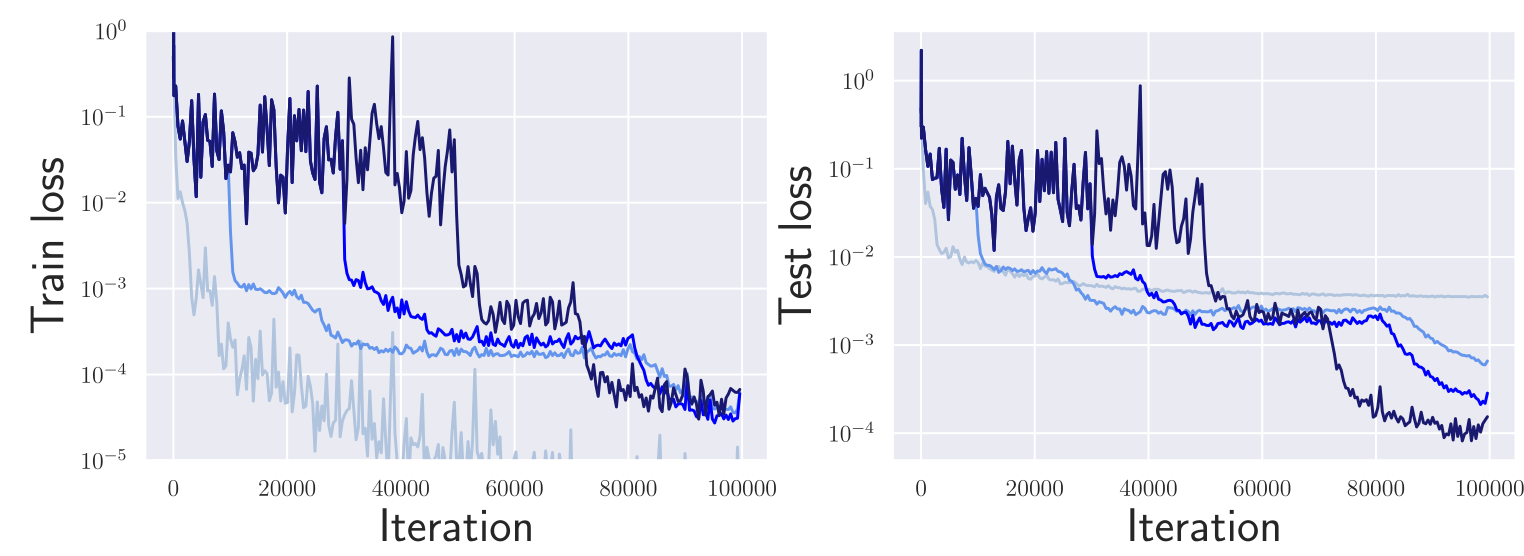
\includegraphics[width=0.8\textwidth]{./pics/dn_loss.png}
    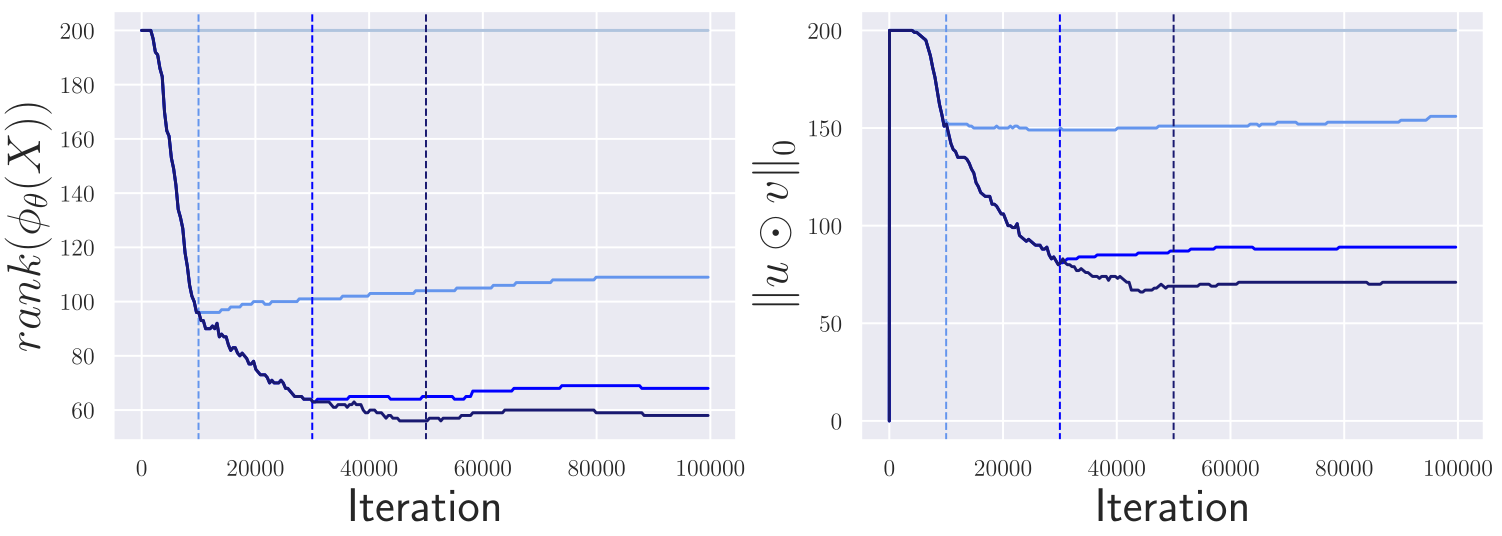
\includegraphics[width=0.8\textwidth]{./pics/dn_sparsity.png}
    
\includegraphics[width=\textwidth]{./pics/dn_setup.png}
    \caption{Diagonal Linear Nets Results \label{fig: diagonal}}
\end{figure}

Figure \ref{fig: digonal} shows the results stated in the previous chapters.
In all three cases of large step size the loss stabilizes and the feature
sparsity progress can be seen on the rank of the Jacobian and feature
sparsity coefficient.



\subsection{Simple ReLU Networks}
\textbf{Two Layer ReLU networks in 1D.}
Considered is a one dimensional regression task with $12$ points. A ReLU
network with 100 neurons with SGD with a long linear warmup followed by a
step size decay at $2\%$ and $50\%$ of iterations respectively. Loss
stabilization is observed at around $10^{-5}$, the predictor becomes simpler
and is expected to generalize better and both the rank and the feature
sparsity coefficient decrease during loss stabilization. Because of the
low dimensionality of the example it can be directly observed that the final
predictor is sparse in terms of the number of distinct ReLU kinks \ref{fig:
relu2}.

\begin{figure}[H]
    \centering
    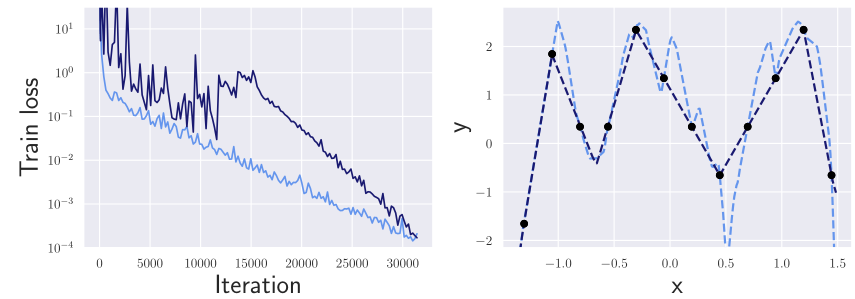
\includegraphics[width=0.8\textwidth]{./pics/relu2_loss.png}
    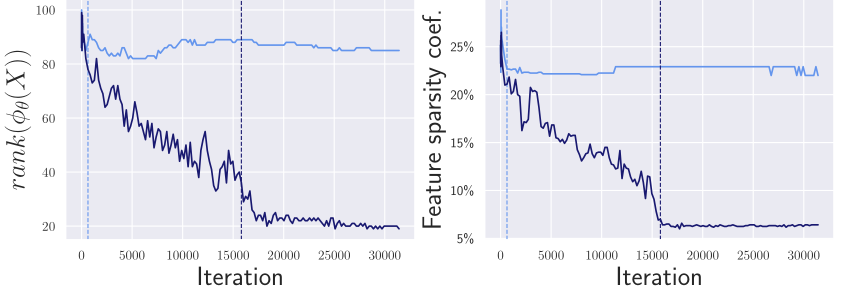
\includegraphics[width=0.8\textwidth]{./pics/relu2_sparsity.png}
    
\includegraphics[width=\textwidth]{./pics/relu2_setup.png}
    \caption{\textbf{Two Layer} ReLU: 1D regression task \label{fig: relu2}}
\end{figure}


\textbf{Three Layer ReLU networks in 1D.}
For deeper ReLU networks a teacher-student setup with a random three layer
teacher ReLU network with 2 neurons at each hidden layer is used. The student
network has 10 neurons on each layer and is trained on $50$ samples. This
kind of setup is useful because it is known that the student network can
implement the ground truth predictor but might not find it due to the small
sample size. The model is trained using SGD with a medium constant step size
and on contrast with a large step size with warmup decayed after $10\%, 30\%$
an $50\%$ of iterations, respectively.

\begin{figure}[H]
    \centering
    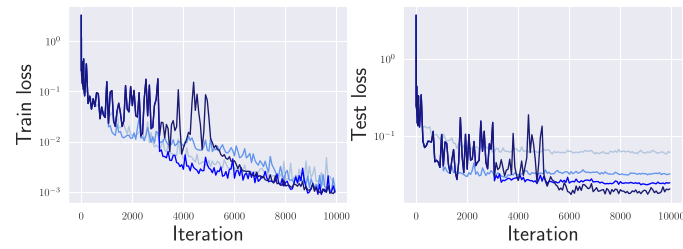
\includegraphics[width=0.8\textwidth]{./pics/relu3_loss.png}
    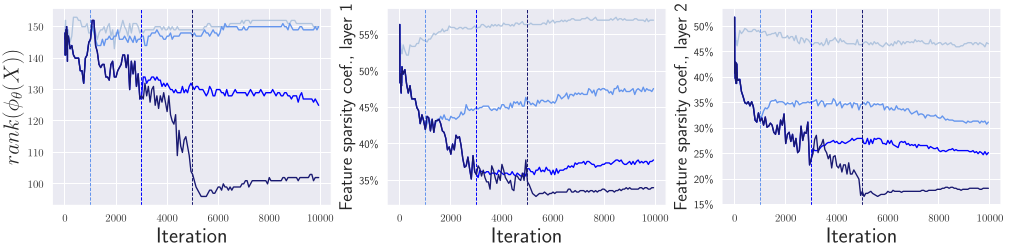
\includegraphics[width=\textwidth]{./pics/relu3_sparsity.png}
    
\includegraphics[width=\textwidth]{./pics/relu3_setup.png}
    \caption{\textbf{Three Layer} ReLU: teacher-student setup \label{ref: relu3}}
\end{figure}

\subsection{Deep ReLU Networks}
In this section a state of the art example is considered to show the sparse
feature learning. Specifically considered is an image classification task,
where the DenseNet-100-12 is trained on CIFAR-10, CIFAR-100 and TinyImageNet
using SGD with batch size $256$ and different step size schedules. An
exponentially increasing step size schedule is used, with exponent $1.05$ to
establish loss stabilization. The rank of the Jacobian cannot be measured
because of too large matrix dimensions, hence only the feature sparsity
coefficient is taken at two layers: end of super block 3 (middle of network)
and super block-block 4 (before average polling at the end of the network) of
DenseNets. Two cases are tested one basic setting and a state of the art
setting with momentum and standard augmentation. In all of the cases the same
observations are made as for the much simpler toy models, i.e. shallow ReLU
networks and diagonal linear nets \ref{fig: deep}

\begin{figure}[H]
    \centering
    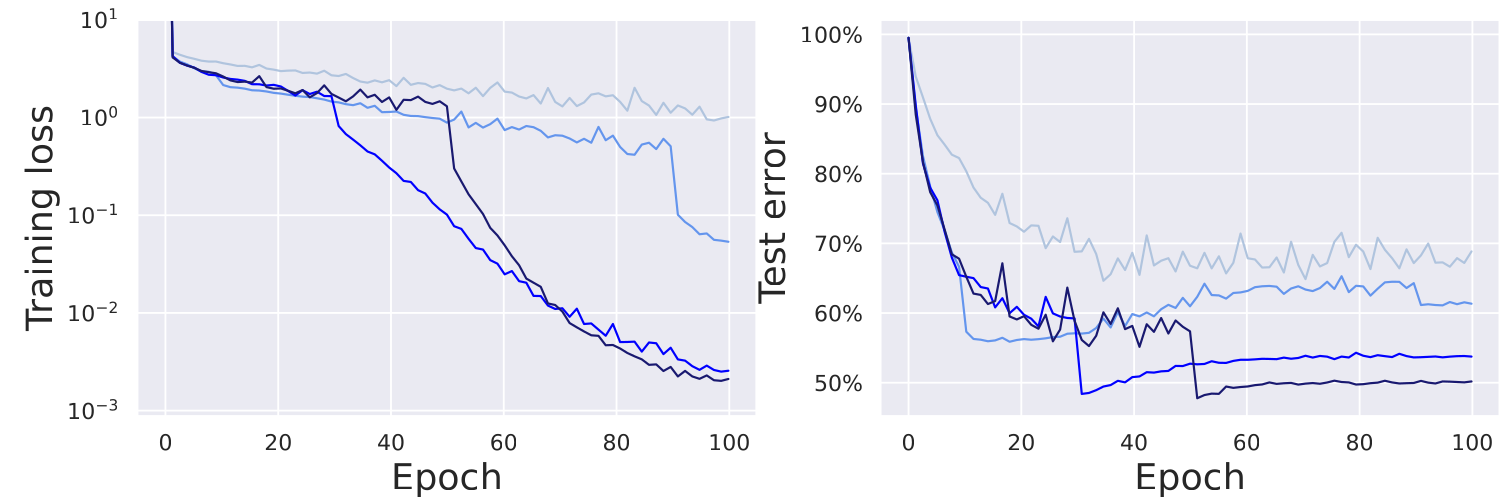
\includegraphics[width=0.8\textwidth]{./pics/densen_tiny_loss.png}
    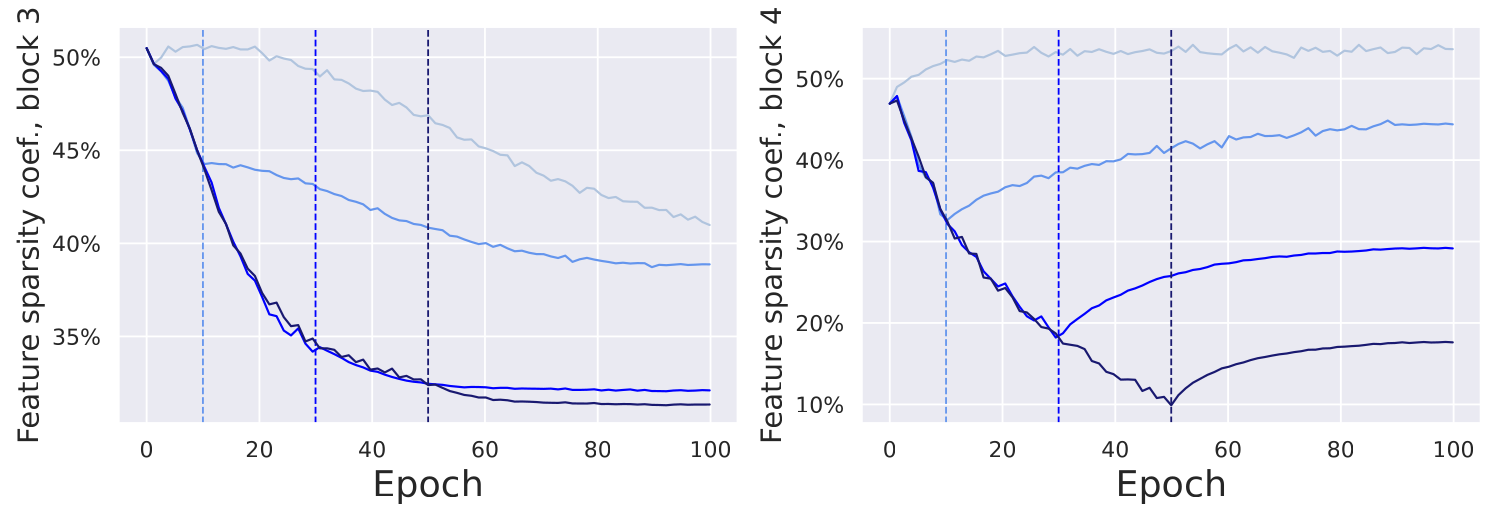
\includegraphics[width=0.8\textwidth]{./pics/densen_tiny_sparsity.png}
    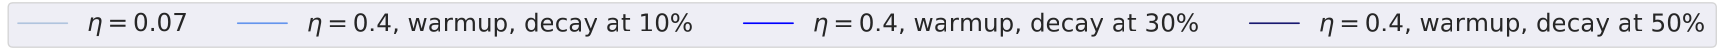
\includegraphics[width=\textwidth]{./pics/densen_tiny_setup.png}
    \caption{\textbf{DenseNet-100} trained on \textbf{ImageNet}
    (Image classification Task) \label{fig: deep}}
\end{figure}


\nocite{andriushchenko2023sgd}
\nocite{shalev2014understanding}
\nocite{pillaudvivien2022label}
\printbibliography

\end{document}
